\documentclass[a4paper,10pt,twocolumn]{jsarticle}
\usepackage{myjlababsstyle}
\begin{document}
\section{システム構成図の例}
システム構成図が論理的に描けると,論文そのものの説明もしやすくなる.
ここでは,シスム構成図の例をいくつか記載する.
\begin{figure}[t]
  \centering
  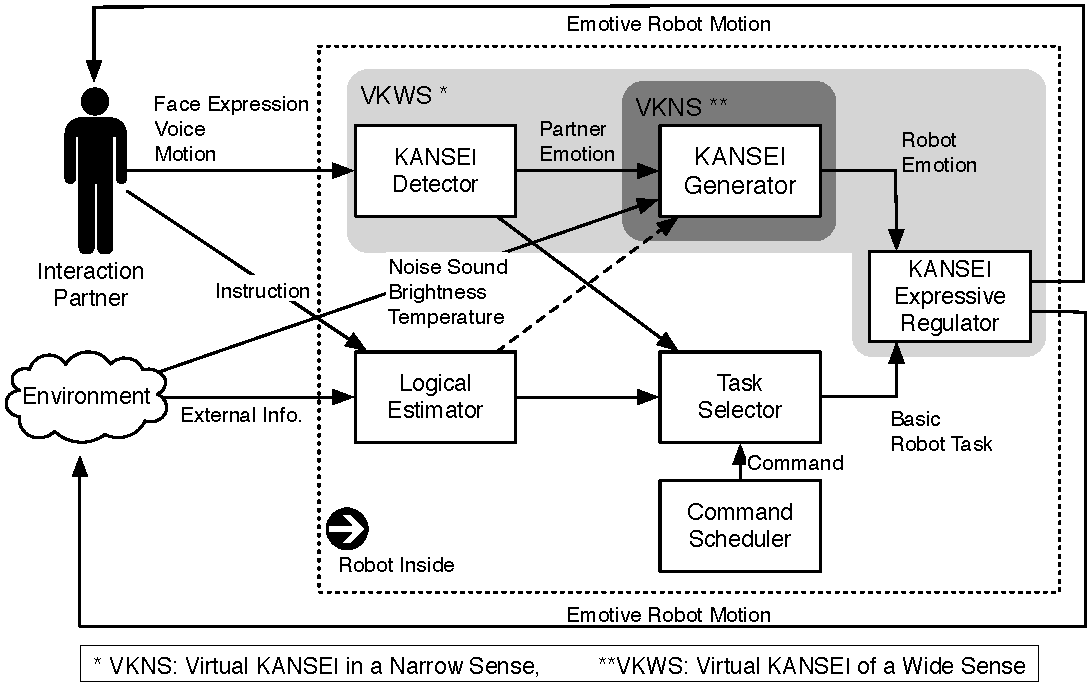
\includegraphics[width=9cm]{VKall.pdf}
  \vspace{-7mm}
  \caption{擬似感性の構成}
  \label{fig:vkall}
  \vspace{5mm}
\end{figure}

\begin{figure}[t]
  \centering
  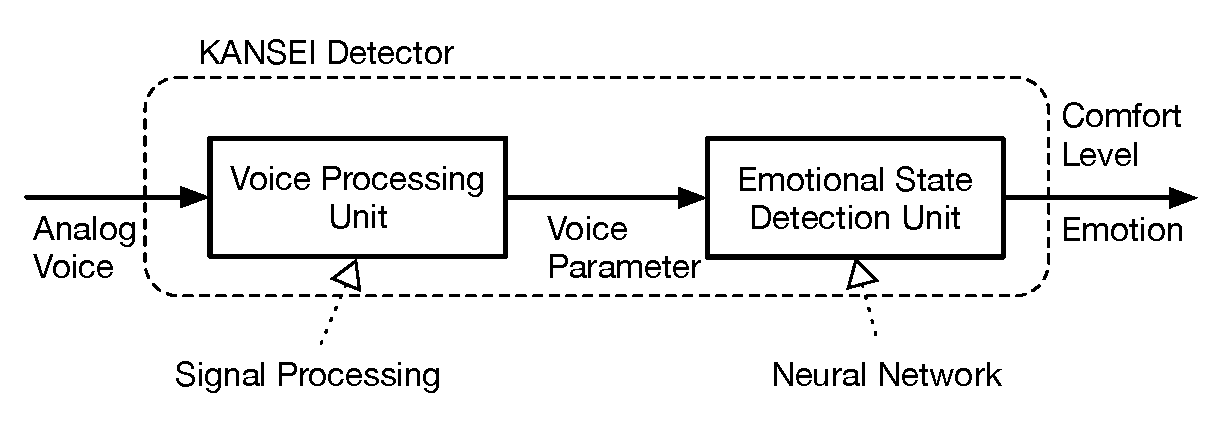
\includegraphics[width=8cm]{VoiceKANSEIDetector.pdf}
  \vspace{-7mm}
  \caption{音声からの感性同定部}
  \label{fig:VoiceKANSEIDetector}
  \vspace{5mm}
\end{figure}

%
\end{document}